% !TeX root = ../main.tex
\chapter{Testowanie i ewaluacja}
\label{chap:evaluation}

% FIRST DRAFT. Sources: test files in the repository, nlp/eval/artifacts
% (gold sets and reports), docs/phase-1-dataflow.md, docs/phase-1-nlp-*.md,
% docs/performance-*.md. The weak-label analysis (Steam voted_up) and the
% case-study numbers were computed while drafting, on 2026-11-23, with
% read-only queries on co_reporting_dev (Appendix A) -- re-run and confirm.

Ten rozdział odpowiada na pytanie, czy system działa i jak dobrze.
Najpierw opisujemy testy oprogramowania, od jednostkowych po pełne przebiegi w chmurze.
Potem oceniamy trzy własności, które zapowiedzieliśmy we wstępie: jakość klasyfikacji, powtarzalność przetwarzania oraz wydajność z kosztami.
Rozdział kończą wyniki studium przypadku i zestawienie kryteriów akceptacji.

\section{Testy jednostkowe i analiza statyczna}
\label{sec:eval-unit}

Kod usług sprawdza \num{304} funkcji testowych, uruchamianych przez \code{pytest} lokalnie i w potoku \ac{cicd} dla każdego zgłoszenia zmian.
Ich rozkład na komponenty przedstawia tabela~\ref{tab:test-counts}.
Liczba przypadków testowych jest większa, bo część testów jest sparametryzowana.

\begin{table}[hbp]
  \caption{Liczba funkcji testowych w poszczególnych komponentach}
  \label{tab:test-counts}
  \centering
  \small
  \begin{tabular}{|l|p{0.5\textwidth}|r|}
    \hline
    Komponent                    & Przykłady sprawdzanych własności                                                           & Testy      \\
    \hline
    \texttt{collectors/}         & determinizm i zależność pseudonimu od soli, zapis paczek, odczyt konfiguracji wydarzeń      & \num{35}   \\
    \hline
    \texttt{publisher/}          & obliczanie przerw, budowa zapytań i komunikatów, instrukcja scalania, walidacja konfiguracji & \num{31}   \\
    \hline
    \texttt{dataflow/}           & walidacja rekordów, budowa wierszy, wykrywanie języka przy współbieżności, budowa grafu      & \num{58}   \\
    \hline
    \texttt{nlp/}                & interfejs klasyfikatora, mapowanie etykiet, przycinanie tekstu, ocena, przygotowanie danych & \num{141}  \\
    \hline
    \texttt{perf/}               & powielanie danych, obliczanie kosztów, zbieranie metryk                                     & \num{39}   \\
    \hline
    \multicolumn{2}{|l|}{Razem}                                                                                                & \num{304}  \\
    \hline
  \end{tabular}
\end{table}

Kilka testów zasługuje na wyróżnienie, bo każdy z nich powstał po konkretnym błędzie.
Testy budowy grafu potoku składają cały graf, łącznie z zapisem do BigQuery, i wychwyciłyby pierwszy z czterech błędów opisanych w podrozdziale~\ref{sec:impl-launch-failures}; ponieważ zapis przez Storage Write API rozwija transformację w Javie, obraz, w którym potok \ac{cicd} uruchamia testy, zawiera środowisko Java.
Test wykrywania języka przywraca bibliotekę \code{langdetect} do stanu sprzed wczytania profili i wywołuje ją z dwunastu wątków jednocześnie, więc nie przejdzie, jeśli ktoś usunie blokadę.
Testy klienta modelu sprawdzają, że recenzja z samych białych znaków dostaje etykietę neutralną z pewnością zero bez wywołania punktu końcowego, a zbyt długi tekst jest przycinany przed wysłaniem.

Poza testami kod przechodzi analizę statyczną: formatowanie \code{black}, reguły \code{ruff} i kontrolę typów \code{mypy} w trybie ścisłym.
Pliki Terraform sprawdzają \code{terraform validate}, \code{tflint} i \code{tfsec}, a widoki raportowe testy danych Dataform: unikalność klucza każdego widoku, warunki na wartościach, zgodność sum każdego widoku z tabelą zdarzeń i brak kolumn z danymi osobowymi.
Celowo zepsute widoki nie przechodziły tych testów, co sprawdziliśmy przed włączeniem automatycznego wdrażania.

\section{Testy integracyjne i systemowe}
\label{sec:eval-system}

Testem systemowym jest u nas pełne odtworzenie, czyli przejście danych od tabeli pośredniej przez kolejkę, potok i scalanie do tabeli zdarzeń.
Takie odtworzenia wykonaliśmy na trzech zbiorach o rosnącej wielkości.
Pierwsze, 5 września 2026~r., objęło \num{4228} komentarzy YouTube: wszystkie trafiły do tabeli zdarzeń, żaden nie trafił do kolejki błędów i żaden nie został bez etykiety.
Drugie, 20 i 21 września, objęło pełny zbiór YouTube, czyli \num{12254} komentarze, najpierw z zaślepką, a potem z modelem XLM-R v2.1.
Trzecie, 18 października, objęło pełny zbiór \num{263893} opinii z obu źródeł.

Przed pierwszym odtworzeniem sprawdziliśmy osobno samą kolejność.
Wydawca opublikował \num{4228} komunikatów, a odczyt wszystkich z subskrypcji kontrolnej z włączonym porządkowaniem nie wykazał ani jednego komunikatu starszego od poprzedniego.
Pierwszy i ostatni czas publikacji zgadzały się z zakresem dat w tabeli pośredniej, a liczba odczytanych komunikatów z liczbą opublikowanych i liczbą wierszy w tabeli.

Testów użytkowych z udziałem osób spoza zespołu nie przeprowadziliśmy w sposób formalny.
\todo[inline]{Testy użytkowe: przeprowadzić z promotorem i 2--3 osobami spoza zespołu scenariusze z przypadków użycia analityka (odczytanie zmian nastrojów wokół wydarzenia, porównanie źródeł) i opisać wyniki; kryterium akceptacji wymaga, by promotor samodzielnie odczytał z panelu zmiany nastrojów.}

\section{Jakość klasyfikacji}
\label{sec:eval-quality}

Jakość modeli mierzyliśmy na zbiorze wzorcowym, czyli na ręcznie oznaczonych komentarzach z naszych danych, oraz na rekomendacjach autorów recenzji Steam.
Główną miarą jest F1 makro, średnia miar F1 dla trzech klas, bo przy nierównych klasach dokładność nagradza model, który dobrze rozpoznaje tylko klasę najliczniejszą.

\subsection{Zbiór wzorcowy w pierwszej wersji}
\label{sec:eval-gold-v1}

Pierwsza wersja zbioru wzorcowego liczyła 300 komentarzy YouTube, wylosowanych z warstwowaniem według źródła i języka, z czego 80 odłożyliśmy jako część kontrolną, która nigdy nie trafia do uczenia.
Klasy były mocno nierówne: 161 komentarzy pozytywnych, 119 neutralnych i tylko 20 negatywnych.
Wyniki trzech kolejnych klasyfikatorów przedstawia tabela~\ref{tab:gold-v1}.

\begin{table}[hbp]
  \caption{Wyniki klasyfikatorów na pierwszej wersji zbioru wzorcowego}
  \label{tab:gold-v1}
  \centering
  \small
  \begin{tabular}{|l|r|r|r|r|}
    \hline
    Klasyfikator                    & \multicolumn{2}{c|}{Część kontrolna (80)} & \multicolumn{2}{c|}{Cały zbiór (300)} \\
    \cline{2-5}
                                    & dokładność  & F1 makro   & dokładność  & F1 makro                       \\
    \hline
    reguła słów kluczowych          & --          & --         & \num{0.417} & \num{0.363}                    \\
    \hline
    DistilBERT v1                   & \num{0.525} & \num{0.498} & \num{0.533} & \num{0.472}                   \\
    \hline
    XLM-R v2                        & \num{0.675} & \num{0.645} & \num{0.913} & \num{0.883}                   \\
    \hline
  \end{tabular}
\end{table}

Wynik XLM-R v2 na całym zbiorze, \num{0.913}, jest mylący i podajemy go tylko dla porządku.
Część treningową zbioru wzorcowego powieliliśmy w danych uczących dziesięciokrotnie, więc model nauczył się jej na pamięć i na niej osiąga wynik \num{1.000}.
Uczciwą miarą uogólniania jest wynik na części kontrolnej: F1 makro wzrosło z \num{0.498} do \num{0.645}.
Na komentarzach angielskich z części kontrolnej, których było tylko 22, nowy model osiągnął F1 makro \num{0.724}, a na pozostałych 58 \num{0.548}.
Model wielojęzyczny poprawił więc wyniki przede wszystkim tam, gdzie angielski model był najsłabszy, choć komentarze nieangielskie wciąż klasyfikuje gorzej.

\subsection{Rozszerzony zbiór wzorcowy}
\label{sec:eval-gold-v3}

Część kontrolna z 80 komentarzy daje bardzo szerokie przedziały ufności, dlatego do porównania wersji v2 i v2.1 rozszerzyliśmy zbiór do 950 komentarzy, z częścią kontrolną liczącą 200.
Wyniki obu wersji na tej części przedstawia tabela~\ref{tab:gold-v3}.

\begin{table}[hbp]
  \caption{Porównanie wersji v2 i v2.1 na części kontrolnej rozszerzonego zbioru wzorcowego (200 komentarzy)}
  \label{tab:gold-v3}
  \centering
  \small
  \begin{tabular}{|l|r|r|r|r|r|r|}
    \hline
    Model & dokładność & F1 makro & F1 pos & F1 neu & F1 neg & F1 makro, angielskie (55) \\
    \hline
    XLM-R v2   & \num{0.590} & \num{0.568} & \num{0.690} & \num{0.533} & \num{0.481} & \num{0.623} \\
    \hline
    XLM-R v2.1 & \num{0.630} & \num{0.600} & \num{0.706} & \num{0.610} & \num{0.485} & \num{0.677} \\
    \hline
  \end{tabular}
\end{table}

Wersja v2.1 spełniła wszystkie trzy warunki wyboru i od 21 września 2026~r. klasyfikuje dane w systemie.
Poprawa nie jest jednak równomierna.
F1 dla klasy negatywnej prawie się nie zmieniło, bo model wymienił czułość na precyzję: v2 rozpoznawał \qty{46.3}{\percent} komentarzy negatywnych z precyzją \num{0.50}, a v2.1 tylko \qty{39.0}{\percent}, ale z precyzją \num{0.64}.
Rozkład błędów wersji v2.1 przedstawia macierz pomyłek w tabeli~\ref{tab:confusion-v21}.

\begin{table}[hbp]
  \caption{Macierz pomyłek wersji v2.1 na części kontrolnej rozszerzonego zbioru wzorcowego}
  \label{tab:confusion-v21}
  \centering
  \small
  \begin{tabular}{|l|r|r|r|r|}
    \hline
    Etykieta wzorcowa & przewidziana pos & przewidziana neu & przewidziana neg & razem \\
    \hline
    pos               & 60               & 19               & 3                & 82    \\
    \hline
    neu               & 21               & 50               & 6                & 77    \\
    \hline
    neg               & 7                & 18               & 16               & 41    \\
    \hline
  \end{tabular}
\end{table}

Najczęstszym błędem jest uznanie komentarza negatywnego za neutralny.
Próbowaliśmy temu zaradzić progiem decyzyjnym: przypisać klasę negatywną, gdy jej prawdopodobieństwo przekroczy próg $T$, a w przeciwnym razie wybrać klasę bardziej prawdopodobną spośród dwóch pozostałych.
Próg dobieraliśmy na części strojenia, a sprawdzaliśmy raz, na części kontrolnej.
Najlepszy na części strojenia próg $T=\num{0.10}$ pogorszył F1 makro na części kontrolnej z \num{0.600} do \num{0.580}, więc zrezygnowaliśmy z niego.
Przyczyna okazała się ciekawsza niż sam wynik.
Spośród 46 pominiętych komentarzy negatywnych z obu części mediana prawdopodobieństwa klasy negatywnej wynosiła \num{0.012}, a tylko trzy przekraczały \num{0.10}.
Model nie waha się przy tych komentarzach, tylko pewnie się myli.
Są to w większości wypowiedzi z ukrytą negacją albo slangiem, na przykład \enquote{Best rpg is kcd2 not e33}, \enquote{AI slop} czy \enquote{Stolen from silksong}, których zrozumienie wymaga znajomości kontekstu.
Lepszym rozwiązaniem niż próg będzie więcej takich przykładów w danych uczących.

Dla porządku warto podać punkt odniesienia: reguła przypisująca każdemu komentarzowi klasę pozytywną osiąga na tej części kontrolnej dokładność \num{0.41}.
Przy 200 komentarzach przedział ufności \qty{95}{\percent} dla dokładności \num{0.63} ma szerokość około $\pm\num{0.067}$, więc różnicę między wersjami v2 i v2.1 należy traktować jako wskazówkę, a nie rozstrzygnięcie.

\subsection{Rekomendacje autorów recenzji Steam}
\label{sec:eval-weak-labels}

Zbiór wzorcowy zawiera wyłącznie komentarze YouTube, a model klasyfikuje głównie recenzje Steam.
Lukę tę wypełnia ocena na słabych etykietach: dla każdej z \num{251639} recenzji porównaliśmy etykietę modelu z rekomendacją autora.
Wynik przedstawia tabela~\ref{tab:weak-confusion}.

\begin{table}[hbp]
  \caption{Etykiety modelu XLM-R v2.1 a rekomendacje autorów recenzji Steam}
  \label{tab:weak-confusion}
  \centering
  \small
  \begin{tabular}{|l|r|r|r|r|}
    \hline
    Rekomendacja autora & model: pos      & model: neu      & model: neg     & razem           \\
    \hline
    poleca              & \num{192323}    & \num{38000}     & \num{7889}     & \num{238212}    \\
    \hline
    nie poleca          & \num{2069}      & \num{3630}      & \num{7728}     & \num{13427}     \\
    \hline
  \end{tabular}
\end{table}

Rekomendacja nie jest etykietą wydźwięku tekstu, bo polecający autor może napisać recenzję pełną zastrzeżeń, ale kierunek obu sygnałów powinien się zgadzać.
I zgadza się: wśród recenzji, którym model przypisał wydźwięk pozytywny albo negatywny, czyli \qty{83.5}{\percent} wszystkich, etykieta modelu zgadza się z rekomendacją w \qty{95.3}{\percent} przypadków.
Etykieta pozytywna jest bardzo pewna: \qty{98.9}{\percent} recenzji, które model uznał za pozytywne, autor rzeczywiście poleca.
Z etykietą negatywną jest gorzej.
Model rozpoznaje jako negatywne \qty{57.6}{\percent} recenzji niepolecających, a połowa jego etykiet negatywnych, \num{7889} z \num{15617}, przypada na recenzje polecające.
Lektura przykładów sugeruje, że są to w dużej mierze recenzje, w których autor poleca grę, ale opisuje głównie jej wady.
\todo{Potwierdzić na próbce recenzji (polecające z etykietą neg) i podać 2--3 przykłady.}
Model jest też ostrożniejszy od autorów: gra ma \qty{94.7}{\percent} rekomendacji, a model uznał za pozytywne \qty{77.3}{\percent} recenzji, większość pozostałych uznając za neutralne.

Ważniejsze od zgodności pojedynczych etykiet jest jednak to, czy model widzi te same zmiany nastrojów co autorzy recenzji.
Tabela~\ref{tab:weak-events} zestawia udział rekomendacji z wskaźnikiem netto modelu w oknach wydarzeń.

\begin{table}[hbp]
  \caption{Udział rekomendacji autorów i wskaźnik netto modelu dla recenzji Steam w oknach wydarzeń}
  \label{tab:weak-events}
  \centering
  \small
  \begin{tabular}{|l|r|r|r|}
    \hline
    Okno                                     & Recenzji       & Udział rekomendacji     & Wskaźnik netto modelu \\
    \hline
    premiera                                 & \num{3915}     & \num{0.938}             & \num{0.685}           \\
    \hline
    spór o tekstury generowane przez AI      & \num{5742}     & \num{0.919}             & \num{0.679}           \\
    \hline
    milion sprzedanych egzemplarzy           & \num{12163}    & \num{0.920}             & \num{0.678}           \\
    \hline
    fala uznania krytyków                    & \num{13715}    & \num{0.962}             & \num{0.742}           \\
    \hline
    The Game Awards 2025                     & \num{4749}     & \num{0.876}             & \num{0.619}           \\
    \hline
    Indie Game Awards odbierają wyróżnienia  & \num{5075}     & \num{0.880}             & \num{0.608}           \\
    \hline
    aktualizacja rocznicowa                  & \num{895}      & \num{0.924}             & \num{0.682}           \\
    \hline
    poza oknami wydarzeń                     & \num{205385}   & \num{0.952}             & \num{0.716}           \\
    \hline
  \end{tabular}
\end{table}

Model i autorzy zgadzają się co do kierunku zmian.
Oba sygnały są najwyższe w okresie uznania krytyków i najniższe wokół grudniowych gal.
Współczynnik korelacji Pearsona między nimi dla ośmiu okien wynosi \num{0.98}, a korelacji rang Spearmana \num{0.95}.
Wcześniej, w dokumentacji zbierania danych, zapisaliśmy prostą zasadę: jeśli model nie zgodzi się z kierunkiem zmian rekomendacji, to model się myli.
Ten test model przeszedł.

Ta sama analiza w podziale na języki pokazuje, gdzie model jest mniej pewny.
Recenzje po chińsku mają najniższy udział rekomendacji, \qty{85.5}{\percent}, i model zgodnie przypisuje im niski wskaźnik netto, \num{0.559}.
Recenzje po koreańsku mają natomiast \qty{93.4}{\percent} rekomendacji, czyli prawie tyle co angielskie, a wskaźnik netto modelu, \num{0.558}, tak samo niski jak dla chińskich, i najniższą zgodność kierunku, \qty{89.7}{\percent} wobec \qty{96.3}{\percent} dla angielskich.
Różnice między językami trzeba więc czytać ostrożnie: część z nich to rzeczywiste różnice w odbiorze gry, a część to różna jakość modelu w różnych językach.

\subsection{Ograniczenia oceny}
\label{sec:eval-quality-limits}

Ocena ma cztery słabości, które chcemy nazwać wprost.
Po pierwsze, zbiór wzorcowy oznaczała w praktyce jedna procedura: wstępne etykiety nadawał asystent oparty na dużym modelu językowym, a człowiek je przeglądał.
Raport zgodności dla 276 przejrzanych komentarzy pokazuje pełną zgodność wstępnych i ostatecznych etykiet, czyli przegląd nie zmienił żadnej etykiety.
Nie wiemy więc, jak bardzo etykiety wzorcowe odzwierciedlają ludzką ocenę, a jak bardzo ocenę modelu, który je zaproponował.
Rzetelniejsza byłaby niezależna ocena części zbioru przez dwie osoby i miara ich zgodności.
Po drugie, zbiór wzorcowy zawiera tylko komentarze YouTube; recenzje Steam ocenialiśmy wyłącznie przez słabe etykiety.
Po trzecie, każdą wersję modelu trenowaliśmy raz, z jednym ziarnem losowym, więc nie znamy rozrzutu wyników między przebiegami.
Po czwarte, część kontrolna z 200 komentarzy daje przedziały ufności szerokie na kilka punktów procentowych.
\todo[inline]{Recenzent oczekuje kilku przebiegów z różnymi ziarnami i mediany wyników (docs/review-criteria.md); przy trenowaniu na CPU to kilka dób pracy maszyny -- rozważyć choćby 3 przebiegi dostrajania v2.1 i niezależne oznaczenie próbki zbioru wzorcowego.}

\section{Poprawność i powtarzalność przetwarzania}
\label{sec:eval-reproducibility}

Najważniejszą obietnicą systemu jest to, że dwa odtworzenia tych samych danych tym samym klasyfikatorem dają ten sam zbiór wierszy.
Sprawdziliśmy ją w trzech sytuacjach.

Z deterministyczną zaślepką dwa odtworzenia \num{4228} komentarzy z 5 września 2026~r., po usunięciu błędów w wykrywaniu języka, dały identyczny odcisk tabeli: $-\num{10329993396494980651}$.
Żaden identyfikator nie różnił się językiem ani wydźwiękiem.
Ten sam odcisk otrzymaliśmy 20 września, uruchamiając odtworzenie zupełnie inną drogą: z wyzwalacza Cloud Build, z obrazem potoku zbudowanym przez potok \ac{cicd} i wskazanym przez skrót, a nie etykietę.
Odcisk przetrwał więc zmianę sposobu uruchamiania, budowania obrazu i odwołania do niego, co jest mocniejszym wynikiem niż dwa odtworzenia z tego samego terminala.
Po czterech odtworzeniach tabela lądowania zawierała duplikaty, a tabela zdarzeń wciąż dokładnie \num{4228} wierszy, co potwierdziło działanie scalania.

Z prawdziwym modelem wynik jest bliski, ale nie identyczny.
W czterech odtworzeniach z 21 września \num{10811} identyfikatorów sklasyfikowano więcej niż raz, a etykieta zmieniła się dla trzech z nich, czyli dla \qty{0.028}{\percent}.
Wnioskowanie na punkcie końcowym jest więc prawie, ale nie bitowo deterministyczne; przyczyny nie badaliśmy.
Wynik mieści się w kryterium akceptacji, które dopuszcza zmianę etykiety dla najwyżej \qty{0.1}{\percent} opinii.

Trzecie sprawdzenie dotyczyło kolejności.
Potok klasyfikuje każdy rekord niezależnie, bez okien czasowych i agregacji, więc kolejność dostarczenia nie powinna wpływać na wynik.
Porównaliśmy \num{256570} identyfikatorów przetworzonych raz w kolejności chronologicznej, z wydawcy, a raz w kolejności mocno przetasowanej: korelacja rang między czasem publikacji a czasem przetworzenia wynosiła odpowiednio \num{1.00} i \num{0.17}.
Etykieta, pewność i język były identyczne dla wszystkich \num{256570} rekordów.
Przy przyszłych agregacjach w oknach czasowych potoku ten test trzeba będzie powtórzyć, bo okna wprowadzają zależność od spóźnionych danych.

W żadnym przebiegu, także w testach wydajności przy największym obciążeniu, nie zginął ani nie zdublował się żaden rekord: liczba różnych identyfikatorów w tabeli docelowej zawsze była równa oczekiwanej.

\section{Wydajność, skalowalność i koszty}
\label{sec:eval-performance}

Badania wydajności zaczęliśmy od dwóch liczb, które już mieliśmy.
Odtworzenia z prawdziwym modelem przetwarzały około 33 opinii na sekundę, a pełny zbiór \num{263893} opinii przechodził przez system w 2 godziny i 12 minut.
Rzeczywisty ruch był przy tym znikomy: najwięcej opinii w ciągu jednej minuty, 49, napisano pod filmami YouTube, co daje \num{0.82} opinii na sekundę, a na Steam najwięcej \num{0.5} na sekundę.
Pytanie nie brzmiało więc, czy system nadąża za tą premierą, tylko jak dużą premierę mógłby obsłużyć i za ile.

\subsection{Przepustowość potoku}
\label{sec:eval-throughput}

Przepustowość mierzyliśmy z zaślepką zamiast modelu, aby zmierzyć potok, a nie punkt końcowy.
Dane z tygodnia premiery, \num{25657} opinii, powieliliśmy dziesięciokrotnie z nowymi identyfikatorami, do \num{256570} rekordów, i zapisywaliśmy wyniki do osobnych tabel, żeby nie trafiły do analizy.
Pierwsze próby mierzyły jednak coś innego niż potok.
Z wydawcą jako źródłem danych potok z jedną i z dwiema maszynami przetwarzał tyle samo, około 50 rekordów na sekundę, a druga maszyna podwajała tylko koszt.
Przyczyną był wydawca: publikuje pod jednym kluczem porządkującym i czeka na potwierdzenie każdej publikacji, więc nie wyśle więcej niż około 50 komunikatów na sekundę.
To świadomy kompromis, bo globalna kolejność jest wymaganiem, ale oznacza, że zwykłe odtworzenie zawsze będzie ograniczone przez wydawcę.

Generator obciążenia uruchomiony z laptopa, publikujący bez porządkowania, okazał się jeszcze wolniejszy: Pub/Sub przyjmował z domowego łącza około 15 komunikatów na sekundę.
Metodą, która zadziałała, było zapełnienie subskrypcji przed uruchomieniem potoku, z generatora działającego w Cloud Build, co dla \num{256570} komunikatów trwało około 2,5 minuty.
Potok, który zastaje pełną kolejkę, przetwarza ją z maksymalną prędkością, niezależnie od tempa publikacji.
Wyniki tej serii przedstawiają tabela~\ref{tab:e1} i rysunek~\ref{fig:throughput}.

\begin{table}[hbp]
  \caption{Przepustowość i koszt potoku z zaślepką przy stałej liczbie maszyn \texttt{e2-standard-2}}
  \label{tab:e1}
  \centering
  \small
  \begin{tabular}{|>{\raggedleft\arraybackslash}p{0.11\textwidth}|>{\raggedleft\arraybackslash}p{0.13\textwidth}|>{\raggedleft\arraybackslash}p{0.1\textwidth}|>{\raggedleft\arraybackslash}p{0.11\textwidth}|>{\raggedleft\arraybackslash}p{0.1\textwidth}|>{\raggedleft\arraybackslash}p{0.15\textwidth}|}
    \hline
    Maszyny (vCPU) & Stan ustalony [rek./s] & Szczyt [rek./s] & Czas zadania [min] & Koszt [USD] & Koszt na \num{1000} rek. [USD] \\
    \hline
    1 (2)          & ok. 345                & 351             & 23                 & \num{0.061} & \num{0.00024}                 \\
    \hline
    2 (4)          & ok. 480                & 488             & 19                 & \num{0.094} & \num{0.00037}                 \\
    \hline
    4 (8)          & ok. 970                & 978             & 14                 & \num{0.092} & \num{0.00036}                 \\
    \hline
  \end{tabular}
\end{table}

\begin{figure}[hbp]
  \centering
  \begin{tikzpicture}
    \begin{axis}[
        font=\footnotesize,
        ybar, bar width=14mm,
        width=0.6\textwidth, height=5.5cm,
        xtick={1,2,3}, xticklabels={1 maszyna, 2 maszyny, 4 maszyny},
        xmin=0.4, xmax=3.6,
        ymin=0, ymax=1150,
        ylabel={rekordy na sekundę},
        nodes near coords, nodes near coords style={font=\footnotesize},
        ymajorgrids, grid style={gray!30},
        enlarge x limits=false]
      \addplot[fill=blue!35, draw=blue!60!black] coordinates {(1,345) (2,480) (3,970)};
    \end{axis}
  \end{tikzpicture}
  \caption{Przepustowość potoku w stanie ustalonym w zależności od liczby maszyn roboczych}
  \label{fig:throughput}
\end{figure}

Przepustowość rośnie z liczbą maszyn: \num{1.4} raza przy przejściu z jednej na dwie i dwukrotnie przy przejściu z dwóch na cztery.
Dlaczego pierwszy krok jest mniejszy, nie wiemy, bo jeden przebieg dla każdej konfiguracji nie pozwala oddzielić rzeczywistego efektu od zmienności między przebiegami.
Każde zadanie spędza około 8--10 minut na uruchamianiu i zatrzymywaniu, więc przy krótkich przebiegach ten stały czas dominuje koszt.
Dlatego cztery maszyny kosztowały tyle samo co dwie: skończyły szybciej.
W porównaniu z rzeczywistym ruchem jedna maszyna ma ponad trzystukrotny zapas, a nawet ograniczony do 50 rekordów na sekundę wydawca pięćdziesięciokrotny.

\subsection{Koszty}
\label{sec:eval-costs}

Koszt przetworzenia tysiąca opinii przez potok pracujący z pełną wydajnością wynosi od \num{0.00024} do \num{0.00037}~USD według cen katalogowych dla regionu warszawskiego.
Za wydawcą, gdy maszyny głównie czekały na dane, ta sama praca kosztowała od \num{0.0011} do \num{0.0024}~USD na tysiąc opinii.
Wszystkie eksperymenty wydajnościowe, łącznie z nieudanymi próbami, kosztowały około \num{1.35}~USD.

Znacznie droższy od potoku jest model.
Replika punktu końcowego na maszynie \code{n1-standard-8} kosztuje \num{0.636}~USD za godzinę, łącznie z opłatą za zarządzanie, a pełne odtworzenie z modelem trwało ponad dwie godziny na dwóch replikach.
Stałym kosztem projektu jest baza serwera MLflow, od 40 do 55~zł miesięcznie.
Największą pojedynczą pozycją okazał się jednak błąd: dyski zatrzymanej maszyny Workbench, około 140~zł miesięcznie, aż do jej usunięcia.

Kosztów nie liczyliśmy z rozliczeń konta, tylko z zużycia zasobów i cennika, bo eksport rozliczeń do BigQuery nie był włączony, a część zespołu nie miała dostępu do konta rozliczeniowego.
\todo[inline]{Do wykonania: pomiar przepustowości z prawdziwym modelem na punkcie końcowym (1, 2 repliki) oraz model kosztów: koszt pełnego odtworzenia, praca ciągła a na żądanie, prognoza dla premiery 10 i 100 razy większej (docs/performance-results.md, E3 i E6).}

\section{Wyniki studium przypadku}
\label{sec:eval-case-study}

System sklasyfikował \num{263893} opinii: \num{251639} recenzji Steam z okresu od 24 kwietnia 2025~r. do 14 października 2026~r. i \num{12254} komentarzy YouTube z okresu od 9 czerwca 2024~r. do 30 kwietnia 2026~r.
\qty{75.9}{\percent} opinii model uznał za pozytywne, \qty{17.3}{\percent} za neutralne i \qty{6.8}{\percent} za negatywne, co daje wskaźnik netto ze wzoru~\eqref{eq:net-sentiment} równy \num{0.691}.
Źródła różnią się jednak już na wejściu.
Recenzje Steam mają wskaźnik netto \num{0.710}, przy \qty{77.3}{\percent} opinii pozytywnych, a komentarze YouTube tylko \num{0.296}, przy \qty{48.4}{\percent} pozytywnych i \qty{18.7}{\percent} negatywnych.
Najprostsze wyjaśnienie jest takie, że recenzję pisze kupujący, który grę zwykle polubił, a pod zwiastunem komentuje każdy, także ten, kto jest nią rozczarowany albo nie zamierza jej kupić.
To kolejny argument za tym, by efekt wydarzenia liczyć względem tła z tego samego źródła.

Przebieg wskaźnika netto w kolejnych tygodniach przedstawia rysunek~\ref{fig:weekly-net}.

\begin{figure}[hbp]
  \centering
  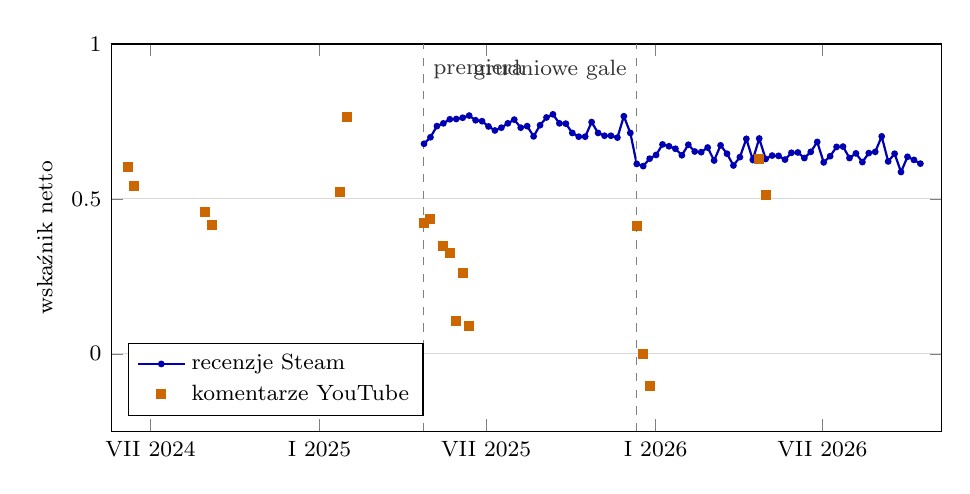
\begin{tikzpicture}
    \begin{axis}[
        font=\footnotesize,
        width=\textwidth, height=6.5cm,
        xmin=2024.38, xmax=2026.85,
        ymin=-0.25, ymax=1.0,
        xtick={2024.4973,2025.0,2025.4959,2026.0,2026.4959},
        xticklabels={VII 2024, I 2025, VII 2025, I 2026, VII 2026},
        ylabel={wskaźnik netto},
        ymajorgrids, grid style={gray!30},
        legend style={at={(0.02,0.04)}, anchor=south west, font=\footnotesize},
        legend cell align=left]
      \addplot[blue!70!black, thick, mark=*, mark size=0.8pt] coordinates {
        (2025.3110,0.678) (2025.3301,0.699) (2025.3493,0.735) (2025.3685,0.744) (2025.3877,0.757) (2025.4068,0.758) (2025.4260,0.762) (2025.4452,0.769) (2025.4644,0.754) (2025.4836,0.751) (2025.5027,0.734) (2025.5219,0.721) (2025.5411,0.730) (2025.5603,0.744) (2025.5795,0.756) (2025.5986,0.730) (2025.6178,0.735) (2025.6370,0.702) (2025.6562,0.738) (2025.6753,0.763) (2025.6945,0.773) (2025.7137,0.744) (2025.7329,0.743) (2025.7521,0.713) (2025.7712,0.701) (2025.7904,0.701) (2025.8096,0.748) (2025.8288,0.713) (2025.8479,0.704) (2025.8671,0.704) (2025.8863,0.698) (2025.9055,0.767) (2025.9247,0.713) (2025.9438,0.613) (2025.9630,0.606) (2025.9822,0.630) (2026.0014,0.642) (2026.0205,0.676) (2026.0397,0.670) (2026.0589,0.662) (2026.0781,0.641) (2026.0973,0.675) (2026.1164,0.653) (2026.1356,0.651) (2026.1548,0.666) (2026.1740,0.624) (2026.1932,0.673) (2026.2123,0.646) (2026.2315,0.608) (2026.2507,0.635) (2026.2699,0.694) (2026.2890,0.626) (2026.3082,0.695) (2026.3274,0.629) (2026.3466,0.640) (2026.3658,0.639) (2026.3849,0.627) (2026.4041,0.649) (2026.4233,0.650) (2026.4425,0.632) (2026.4616,0.652) (2026.4808,0.684) (2026.5000,0.618) (2026.5192,0.638) (2026.5384,0.668) (2026.5575,0.669) (2026.5767,0.632) (2026.5959,0.647) (2026.6151,0.619) (2026.6342,0.648) (2026.6534,0.652) (2026.6726,0.702) (2026.6918,0.621) (2026.7110,0.646) (2026.7301,0.587) (2026.7493,0.636) (2026.7685,0.626) (2026.7877,0.614)};
      \addlegendentry{recenzje Steam}
      \addplot[orange!80!black, only marks, mark=square*, mark size=1.6pt] coordinates {
        (2024.4304,0.602) (2024.4495,0.543) (2024.6599,0.457) (2024.6790,0.417) (2025.0616,0.522) (2025.0808,0.764) (2025.3110,0.421) (2025.3301,0.435) (2025.3685,0.349) (2025.3877,0.326) (2025.4068,0.106) (2025.4260,0.261) (2025.4452,0.091) (2025.9438,0.414) (2025.9630,-0.001) (2025.9822,-0.104) (2026.3082,0.628) (2026.3274,0.514)};
      \addlegendentry{komentarze YouTube}
      \draw[gray, dashed] (axis cs:2025.3096,-0.25) -- (axis cs:2025.3096,1.0);
      \draw[gray, dashed] (axis cs:2025.9425,-0.25) -- (axis cs:2025.9425,1.0);
      \node[anchor=north west, font=\footnotesize, gray!40!black] at (axis cs:2025.3096,0.98) {premiera};
      \node[anchor=north east, font=\footnotesize, gray!40!black] at (axis cs:2025.9425,0.98) {grudniowe gale};
    \end{axis}
  \end{tikzpicture}
  \caption{Tygodniowy wskaźnik wydźwięku netto według źródeł; pokazano tygodnie z co najmniej 20 opiniami}
  \label{fig:weekly-net}
\end{figure}

Wykres pokazuje trzy rzeczy.
Po pierwsze, nastroje na Steam rosły przez pierwsze tygodnie po premierze, od \num{0.68} w tygodniu premiery do \num{0.77} w czerwcu 2025~r., co zgadza się z falą uznania krytyków.
Po drugie, grudzień 2025~r. przyniósł na Steam wyraźny i trwały spadek, z \num{0.71} do \num{0.61}, a wskaźnik do końca okresu nie wrócił do poziomu sprzed gal i w 2026~r. utrzymywał się w przedziale od \num{0.59} do \num{0.70}.
Po trzecie, komentarze YouTube reagują znacznie silniej niż recenzje: w grudniu wskaźnik spadł z \num{0.41} do $-\num{0.10}$.
Na YouTube każde wydarzenie to inny zestaw filmów, więc część tej zmienności wynika z doboru materiału, a nie tylko z nastrojów.

Na wykresie widać też jedną anomalię.
W tygodniu rozpoczynającym się 24 listopada 2025~r. na Steam napisano \num{30653} recenzje, dziesięć razy więcej niż w sąsiednich tygodniach, ze wskaźnikiem netto \num{0.767}.
Ten tydzień nie wiąże się z żadnym z dwunastu wydarzeń w konfiguracji.
\todo{Ustalić przyczynę skoku liczby recenzji w tygodniu od 24.11.2025 (np. promocja w sklepie lub nominacje do nagród) i rozważyć dodanie wydarzenia.}

Efekt poszczególnych wydarzeń względem tła z tego samego źródła przedstawia rysunek~\ref{fig:event-lift}.

\begin{figure}[hbp]
  \centering
  \begin{tikzpicture}
    \begin{axis}[
        font=\footnotesize,
        xbar, bar width=2.4mm,
        width=0.62\textwidth, height=9.5cm,
        y dir=reverse,
        symbolic y coords={reveal,flying,dd,launch,ai,million,critical,tga,iga,anniv},
        ytick={reveal,flying,dd,launch,ai,million,critical,tga,iga,anniv},
        yticklabels={zapowiedź, zwiastun \enquote{Flying Waters}, Xbox Developer Direct, premiera, spór o tekstury AI, milion egzemplarzy, uznanie krytyków, The Game Awards 2025, Indie Game Awards, aktualizacja rocznicowa},
        xmin=-0.65, xmax=0.4,
        xlabel={zmiana wskaźnika netto względem tła},
        xmajorgrids, grid style={gray!30},
        enlarge y limits=0.06,
        legend style={at={(0.02,0.98)}, anchor=north west, font=\footnotesize},
        legend cell align=left]
      \addplot[fill=blue!45, draw=blue!60!black] coordinates {
        (-0.026,launch) (-0.032,ai) (-0.034,million) (0.034,critical) (-0.094,tga) (-0.104,iga) (-0.029,anniv)};
      \addlegendentry{Steam}
      \addplot[fill=orange!60, draw=orange!70!black] coordinates {
        (0.302,reveal) (0.179,flying) (0.307,dd) (0.139,launch) (0.137,million) (-0.044,critical) (0.163,tga) (-0.566,iga) (0.295,anniv)};
      \addlegendentry{YouTube}
      \draw[black] (axis cs:0,reveal) -- (axis cs:0,anniv);
    \end{axis}
  \end{tikzpicture}
  \caption{Efekt wydarzeń: różnica wskaźnika netto w oknie wydarzenia i w tle z tego samego źródła}
  \label{fig:event-lift}
\end{figure}

Na Steam najsilniejszy negatywny efekt miały dwa grudniowe wydarzenia: wokół The Game Awards wskaźnik był o \num{0.094} niższy od tła, a wokół decyzji Indie Game Awards o \num{0.104}.
Jedynym oknem lepszym od tła była fala uznania krytyków, z różnicą \num{0.034}.
Premiera i kilka dni po niej to przede wszystkim lawina opinii, z liczbą recenzji na dzień \num{8.5} raza większą niż w tle, przy niemal niezmienionym wydźwięku.

Na YouTube największy efekt w całym zbiorze ma decyzja Indie Game Awards: wskaźnik netto spadł do $-\num{0.108}$ wobec \num{0.458} w tle, czyli o \num{0.566}.
To jedyne wydarzenie, przy którym komentarze negatywne przeważyły nad pozytywnymi.
Najlepiej przyjęte były zapowiedź gry, pokaz na Xbox Developer Direct i aktualizacja rocznicowa, z efektem około $+\num{0.30}$.
Ciekawy jest przypadek The Game Awards, przy którym źródła rozjechały się w przeciwnych kierunkach: komentarze pod filmami z gali były lepsze od tła YouTube o \num{0.163}, a recenzje Steam z tego okresu gorsze od tła Steam o \num{0.094}.
Jedno z możliwych wyjaśnień jest takie, że komentujący materiały z gali świętowali zwycięstwa, a recenzje z tego samego okresu pisały w dużej części osoby, które sięgnęły po grę pod wpływem nagród i oceniały ją surowiej.
To hipoteza, której nasze dane nie rozstrzygają.

Zestawienie z rekomendacjami autorów z podrozdziału~\ref{sec:eval-weak-labels} wzmacnia te obserwacje dla Steam, bo spadek wokół grudniowych gal widać także w deklaracjach autorów, niezależnych od modelu: udział rekomendacji spadł z \qty{96.2}{\percent} w okresie uznania krytyków do \qty{87.6}{\percent} wokół The Game Awards.

\section{Spełnienie kryteriów akceptacji}
\label{sec:eval-acceptance}

Tabela~\ref{tab:acceptance} zestawia kryteria akceptacji ze specyfikacji wymagań z wynikami opisanymi w tym rozdziale.

\begin{table}[hbp]
  \caption{Kryteria akceptacji i stan ich spełnienia}
  \label{tab:acceptance}
  \centering
  \small
  \begin{tabular}{|p{0.27\textwidth}|p{0.47\textwidth}|p{0.13\textwidth}|}
    \hline
    Kryterium                          & Wynik                                                                                                                & Stan          \\
    \hline
    przebieg od źródła do panelu       & \num{263893} opinii z dwóch źródeł w tabeli zdarzeń, bez błędnych komunikatów, wyniki na panelu; brak formalnego pokazu dla promotora & częściowo \\
    \hline
    test powtarzalności                & identyczny odcisk dla zaślepki; zmiana etykiety dla \qty{0.028}{\percent} opinii przy modelu (próg \qty{0.1}{\percent})   & spełnione     \\
    \hline
    raport jakości modelu              & ocena na części kontrolnej zbioru wzorcowego i na rekomendacjach autorów Steam, porównanie z poprzednimi wersjami       & spełnione     \\
    \hline
    zgodność infrastruktury z kodem    & do potwierdzenia przed złożeniem pracy                                                                                & do sprawdzenia \\
    \hline
  \end{tabular}
\end{table}

\todo[inline]{Uruchomić terraform plan na środowisku dev i wpisać wynik do tabeli; zorganizować pokaz panelu dla promotora.}
Podsumowanie tego, co z tych wyników wynika dla celu pracy, zawiera następny rozdział.
